\PassOptionsToPackage{unicode=true}{hyperref} % options for packages loaded elsewhere
\PassOptionsToPackage{hyphens}{url}
%
\documentclass[ignorenonframetext,]{beamer}
\usepackage{pgfpages}
\setbeamertemplate{caption}[numbered]
\setbeamertemplate{caption label separator}{: }
\setbeamercolor{caption name}{fg=normal text.fg}
\beamertemplatenavigationsymbolsempty
\usepackage{lmodern}
\usepackage{amssymb,amsmath}
\usepackage{ifxetex,ifluatex}
\usepackage{fixltx2e} % provides \textsubscript
\ifnum 0\ifxetex 1\fi\ifluatex 1\fi=0 % if pdftex
  \usepackage[T1]{fontenc}
  \usepackage[utf8]{inputenc}
  \usepackage{textcomp} % provides euro and other symbols
\else % if luatex or xelatex
  \usepackage{unicode-math}
  \defaultfontfeatures{Ligatures=TeX,Scale=MatchLowercase}
\fi
\usecolortheme{seahorse}
\usefonttheme{structurebold}
% use upquote if available, for straight quotes in verbatim environments
\IfFileExists{upquote.sty}{\usepackage{upquote}}{}
% use microtype if available
\IfFileExists{microtype.sty}{%
\usepackage[]{microtype}
\UseMicrotypeSet[protrusion]{basicmath} % disable protrusion for tt fonts
}{}
\IfFileExists{parskip.sty}{%
\usepackage{parskip}
}{% else
\setlength{\parindent}{0pt}
\setlength{\parskip}{6pt plus 2pt minus 1pt}
}
\usepackage{hyperref}
\hypersetup{
            pdftitle={Panel de comunidades 4: Desarrollo de recursos - The Carpentries},
            pdfborder={0 0 0},
            breaklinks=true}
\urlstyle{same}  % don't use monospace font for urls
\newif\ifbibliography
\usepackage{graphicx,grffile}
\makeatletter
\def\maxwidth{\ifdim\Gin@nat@width>\linewidth\linewidth\else\Gin@nat@width\fi}
\def\maxheight{\ifdim\Gin@nat@height>\textheight\textheight\else\Gin@nat@height\fi}
\makeatother
% Scale images if necessary, so that they will not overflow the page
% margins by default, and it is still possible to overwrite the defaults
% using explicit options in \includegraphics[width, height, ...]{}
\setkeys{Gin}{width=\maxwidth,height=\maxheight,keepaspectratio}
% Prevent slide breaks in the middle of a paragraph:
\widowpenalties 1 10000
\raggedbottom
\setbeamertemplate{part page}{
\centering
\begin{beamercolorbox}[sep=16pt,center]{part title}
  \usebeamerfont{part title}\insertpart\par
\end{beamercolorbox}
}
\setbeamertemplate{section page}{
\centering
\begin{beamercolorbox}[sep=12pt,center]{part title}
  \usebeamerfont{section title}\insertsection\par
\end{beamercolorbox}
}
\setbeamertemplate{subsection page}{
\centering
\begin{beamercolorbox}[sep=8pt,center]{part title}
  \usebeamerfont{subsection title}\insertsubsection\par
\end{beamercolorbox}
}
\AtBeginPart{
  \frame{\partpage}
}
\AtBeginSection{
  \ifbibliography
  \else
    \frame{\sectionpage}
  \fi
}
\AtBeginSubsection{
  \frame{\subsectionpage}
}
\setlength{\emergencystretch}{3em}  % prevent overfull lines
\providecommand{\tightlist}{%
  \setlength{\itemsep}{0pt}\setlength{\parskip}{0pt}}
\setcounter{secnumdepth}{0}

% set default figure placement to htbp
\makeatletter
\def\fps@figure{htbp}
\makeatother

\setbeamertemplate{navigation symbols}{}
\setbeamertemplate{footline}[page number]

\title{Panel de comunidades 4: Desarrollo de recursos - The Carpentries}
\author{Rayna M. Harris @raynamharris\\
~\\
Florencia D'Andrea @cantoflor\_87\\}
\date{4 Septiembre 2018\\
LatinR, Buenos Aires}

\begin{document}
\frame{\titlepage}

\begin{frame}{La programación es importante porque nos permite
automatizar tareas.}
\protect\hypertarget{la-programacion-es-importante-porque-nos-permite-automatizar-tareas.}{}

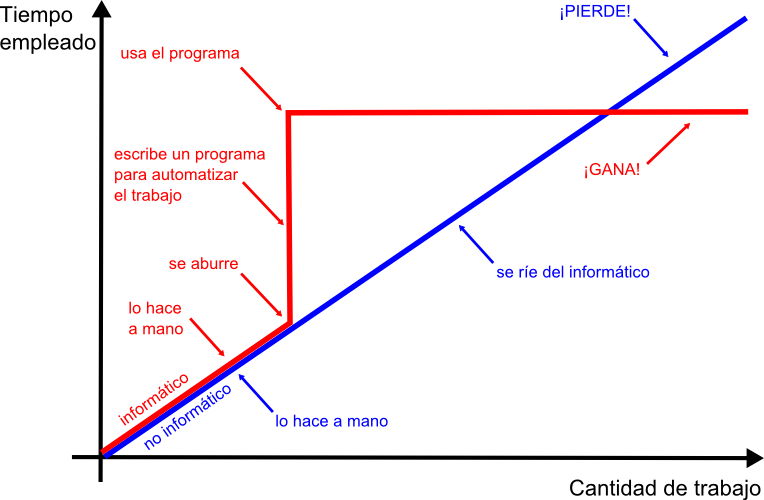
\includegraphics[width=0.75\textwidth,height=\textheight]{../figures/10_talk/trabajo-tiempo-8.png}
\footnote<.->{\url{http://www.mclibre.org/consultar/python/otros/lenguajes-programacion.html}}

\end{frame}

\begin{frame}{R permite generar estadísticas reproducibles y visualizar
datos}
\protect\hypertarget{r-permite-generar-estadisticas-reproducibles-y-visualizar-datos}{}

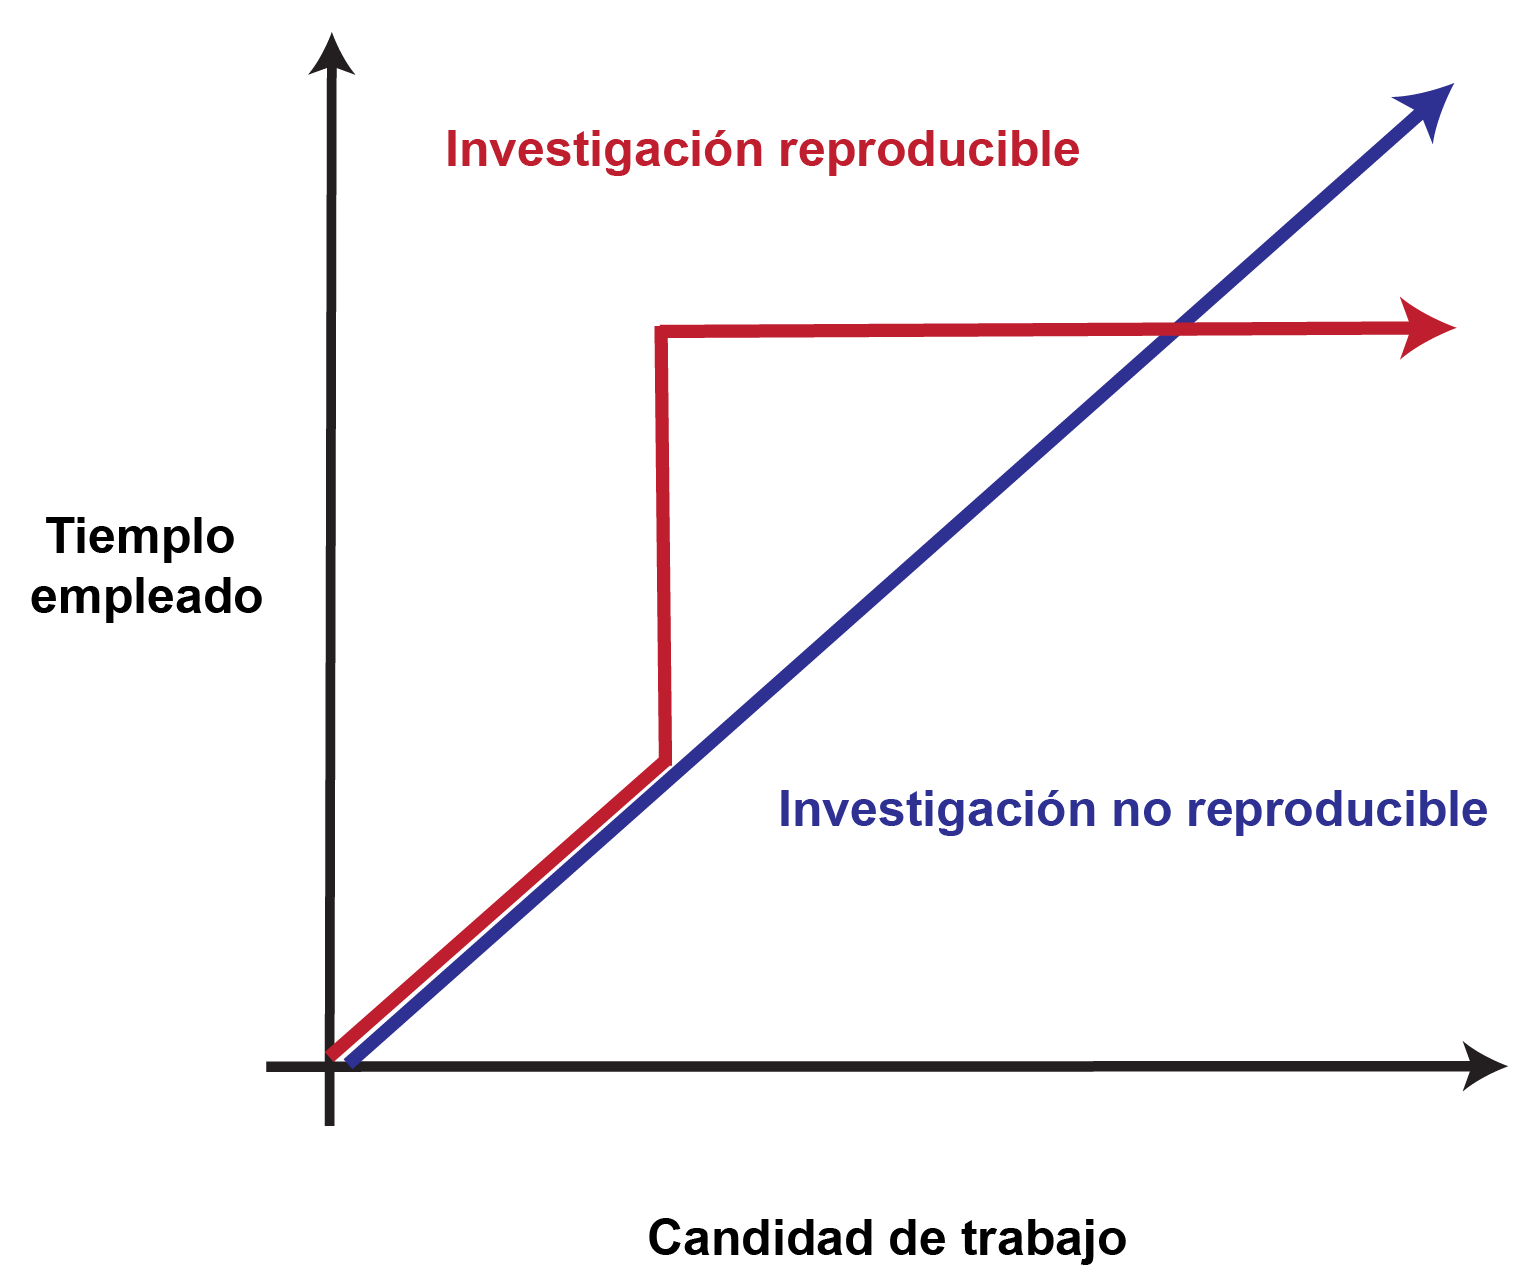
\includegraphics[width=0.75\textwidth,height=\textheight]{../figures/10_talk/tiempo-01.png}

\end{frame}

\begin{frame}{Software Carpentry and Data Carpentry}
\protect\hypertarget{software-carpentry-and-data-carpentry}{}


\includegraphics{../figures/10_talk/swc1.png}


\includegraphics{../figures/10_talk/dc-1.png}


\includegraphics{../figures/10_talk/carpentries-1.png}

\end{frame}

\begin{frame}{La enseñanza colaborativa también ahorra tiempo, ya que
implica una menor cantidad de trabajo}
\protect\hypertarget{la-ensenanza-colaborativa-tambien-ahorra-tiempo-ya-que-implica-una-menor-cantidad-de-trabajo}{}

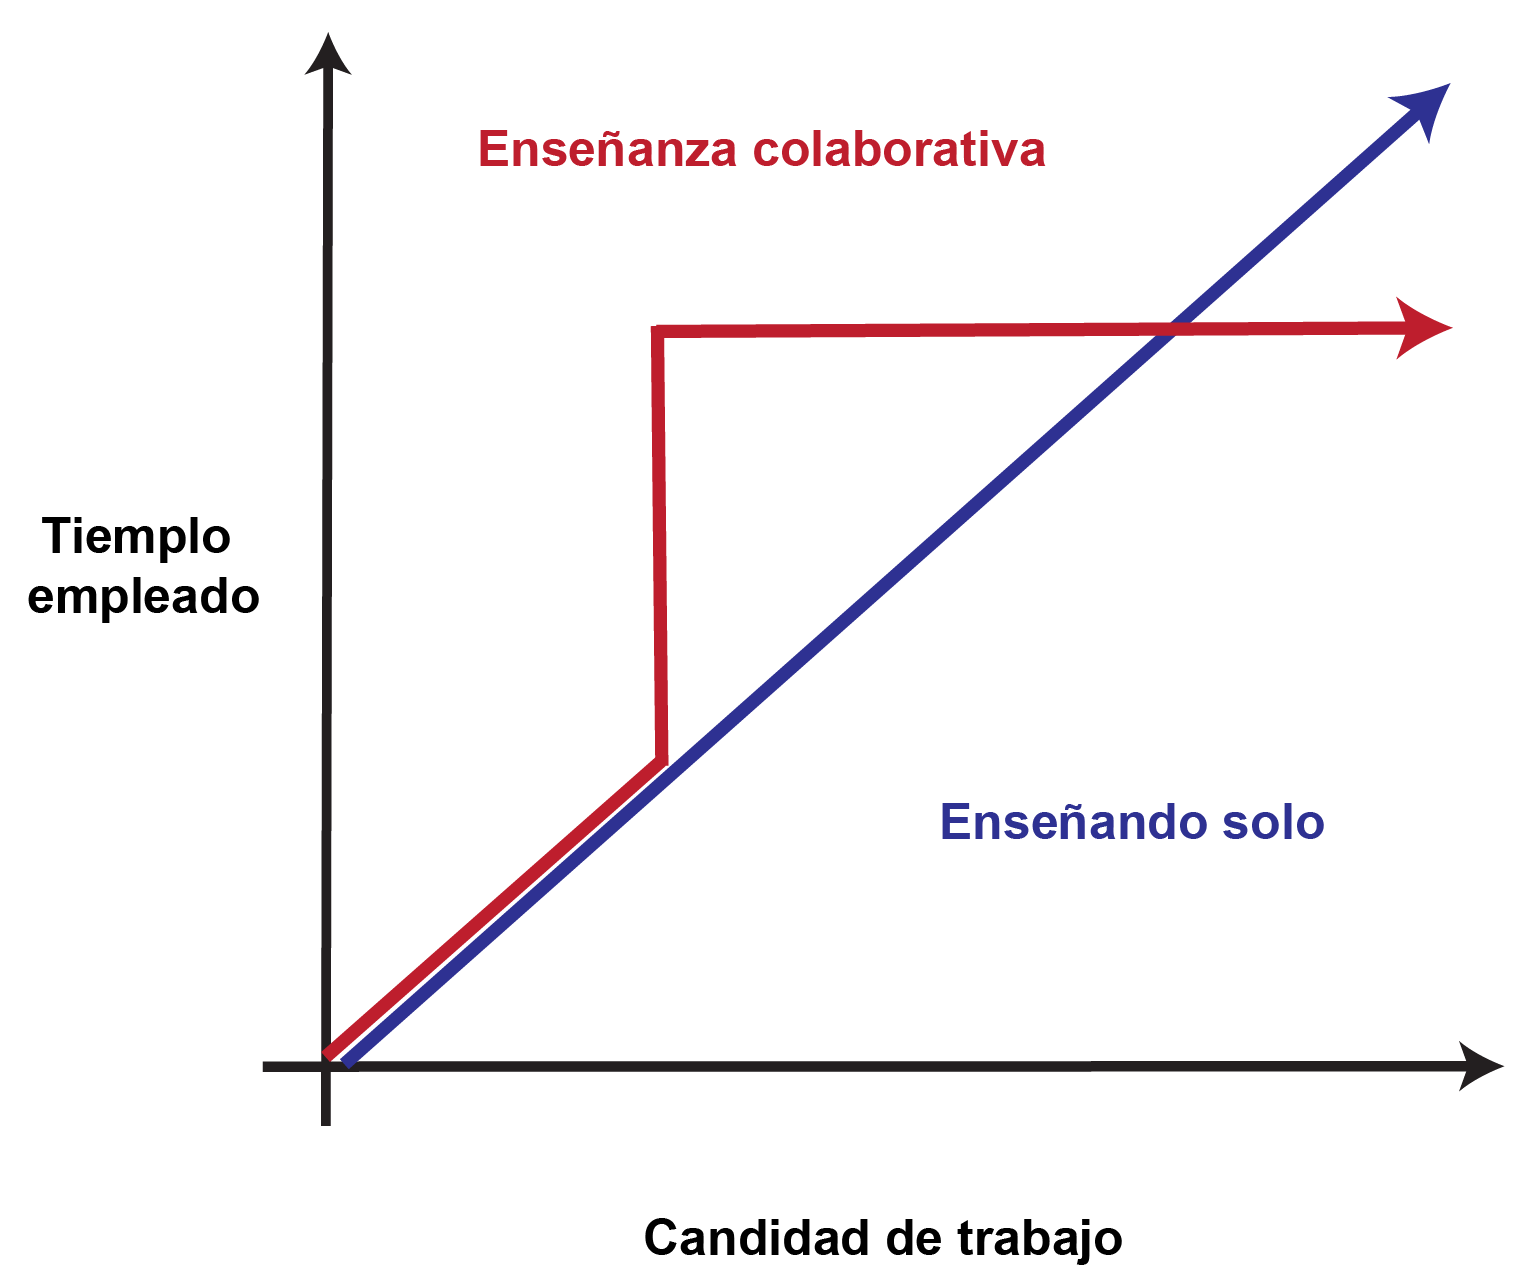
\includegraphics[width=0.75\textwidth,height=\textheight]{../figures/10_talk/tiempo-02.png}

\end{frame}

\begin{frame}{Desarrollo colaborativo de la lección}
\protect\hypertarget{desarrollo-colaborativo-de-la-leccion}{}

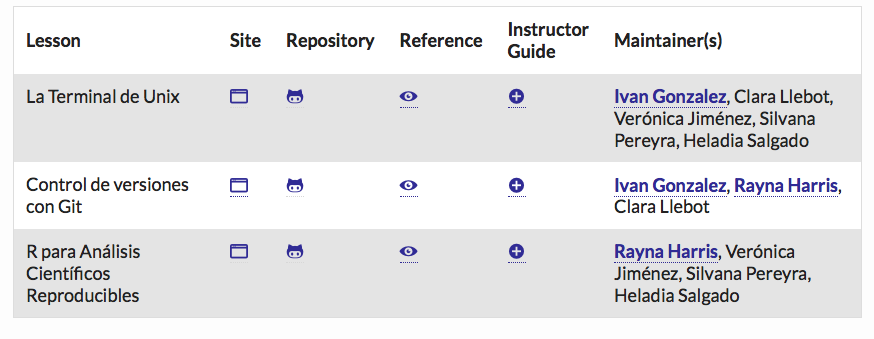
\includegraphics{../figures/10_talk/swc4.png} \footnote<.->{\url{https://software-carpentry.org/lessons/}}

\end{frame}

\begin{frame}{Los materiales se encuentran abiertos y disponibles bajo
la licencia Creative Commons Attribution}
\protect\hypertarget{los-materiales-se-encuentran-abiertos-y-disponibles-bajo-la-licencia-creative-commons-attribution}{}

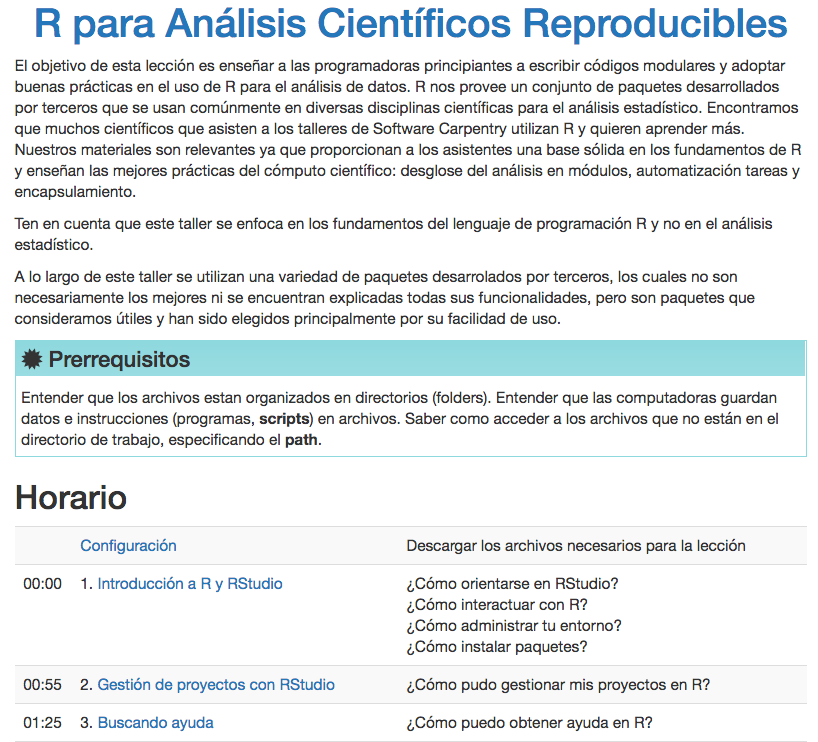
\includegraphics{../figures/10_talk/R-gapminder-es.png}

\end{frame}

\begin{frame}{¿Cómo desarrollamos las lecciones de forma colaborativa?}
\protect\hypertarget{como-desarrollamos-las-lecciones-de-forma-colaborativa}{}

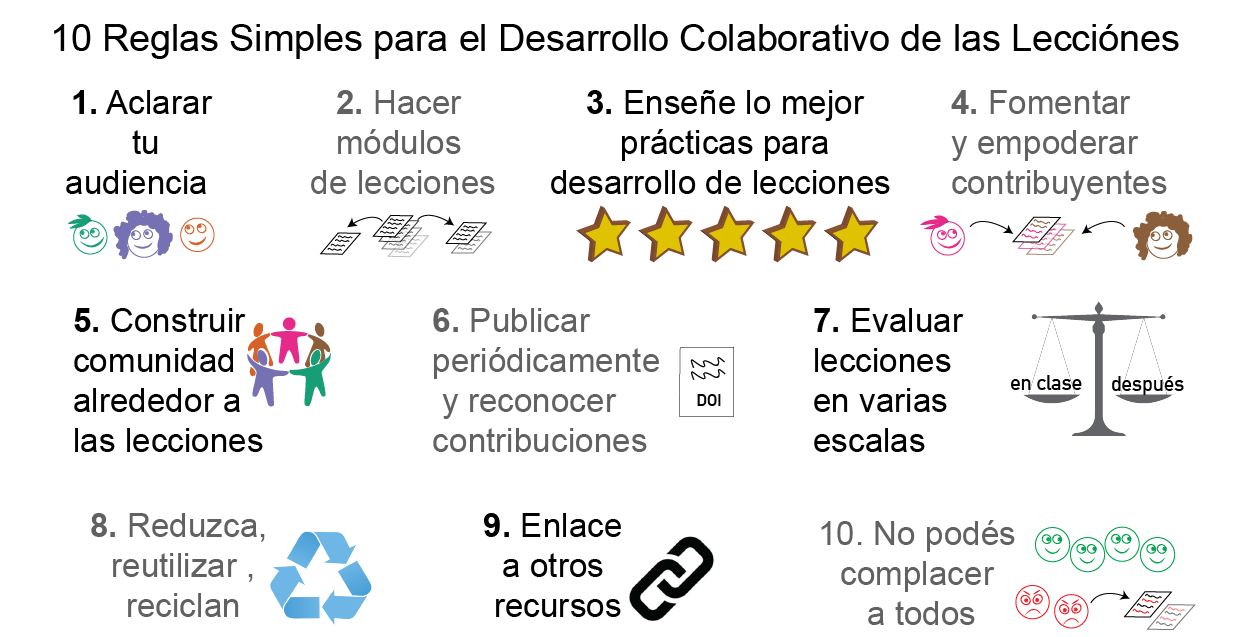
\includegraphics{../figures/10_talk/figure1_es.png}

\footnote<.->{Devenyi et al.~2018 PLOS Comp Bio
  \url{http://journals.plos.org/ploscompbiol/article?id=10.1371/journal.pcbi.1005963}}

\end{frame}

\begin{frame}{Además, enseñamos cómo enseñar mejor}
\protect\hypertarget{ademas-ensenamos-como-ensenar-mejor}{}

\begin{itemize}[<+->]
\tightlist
\item
  Taller mananña: \url{http://latin-r.com/cronograma/\#session-25}
  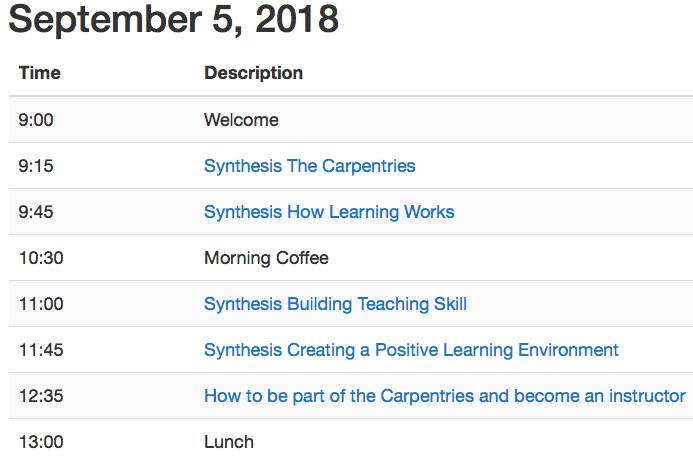
\includegraphics[width=0.75\textwidth,height=\textheight]{../figures/10_talk/LatinRtaller.png}
  \footnote<.->{\url{https://raynamharris.github.io/2018-08-18-ttt-LatinAmerica/}}
\end{itemize}

\end{frame}

\begin{frame}{Hay instructoras certificadas en todo casi todo el mundo}
\protect\hypertarget{hay-instructoras-certificadas-en-todo-casi-todo-el-mundo}{}

\begin{itemize}[<+->]
\tightlist
\item
  Aplicá aquí: \url{http://carpentries.github.io/instructor-training/}
\item
  Usa el \textbf{Group Name} ``LatinR''
\end{itemize}

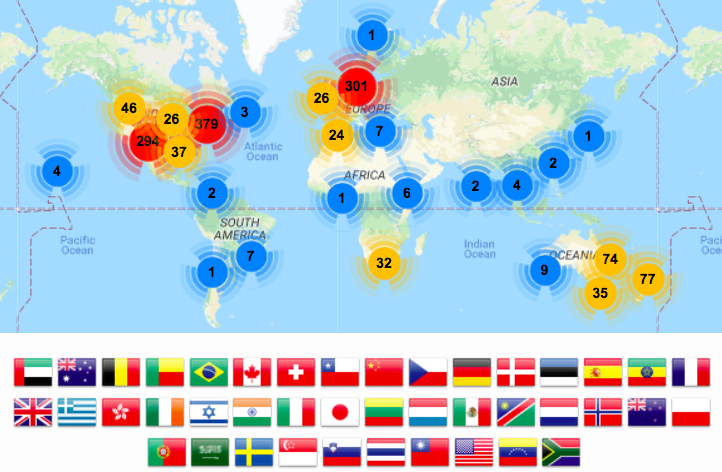
\includegraphics[width=0.75\textwidth,height=\textheight]{../figures/10_talk/joinus.png}
\footnote<.->{\url{https://software-carpentry.org/team/}}

\end{frame}

\begin{frame}{Organizar unos talleres en el futuro}
\protect\hypertarget{organizar-unos-talleres-en-el-futuro}{}

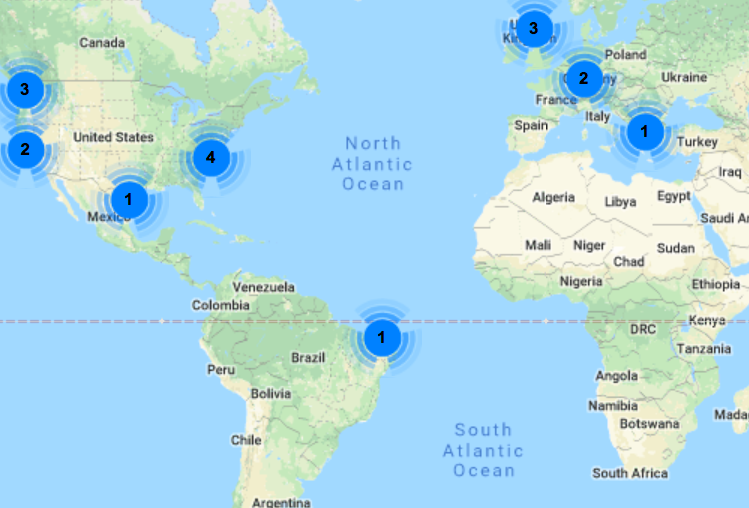
\includegraphics[width=0.75\textwidth,height=\textheight]{../figures/10_talk/workshops2.png}

\footnote<.->{\url{https://software-carpentry.org/workshops/}}

\end{frame}

\begin{frame}{Algunos pensamientos para concluir}
\protect\hypertarget{algunos-pensamientos-para-concluir}{}

\begin{itemize}[<+->]
\tightlist
\item
  Creo que todos aprenden más cuando la ciencia y la educación son
  abiertas y reproducibles
\item
  La mejor manera de aprender es enseñando
\item
  Recuerda que nadie es re buena al principio, pero todas mejoramos con
  la práctica
\end{itemize}

\end{frame}

\begin{frame}{¡Gracias por tu atención! ¡Mantengámonos en contacto!}
\protect\hypertarget{gracias-por-tu-atencion-mantengamonos-en-contacto}{}

Rayna M. Harris @raynamharris

Florencia D'Andrea @cantoflor\_87

Diapositivas acá\footnote<.->{\url{https://github.com/raynamharris/FMR1CA1rnaseq}}
y acá\footnote<.->{\url{https://speakerdeck.com/raynamharris/}}

\end{frame}

\end{document}
